\documentclass{article}
\usepackage{graphicx}
\def\til{\texttt{\~}}

\title{\textbf{2025 Introduction to Computer Software Systems Lab Assignment
\#2}}
\date{September 15, 2025}
\author{Doyoung Kim}

\begin{document}
\maketitle

In this assignment, we implement fundamental operations in the two's complement 
integer and floating-point systems using the C programming language. In order to 
accomplish this, it requires the following six functions to be implemented under 
a specific set of constraints:

\begin{enumerate}
    \item[\texttt{negate}] Implement the negation operator in the two's 
    complement system.
    \item[\texttt{isLess}] Compare two signed integers, returning true if the 
    first argument is less than the second.
    \item[\texttt{float\_abs}] Compute the absolute value of a floating-point
    number using only integer operations.
    \item[\texttt{float\_twice}] Double a floating-point number by manipulating 
    its bit-level representation.
    \item[\texttt{float\_i2f}] Implement the casting operation from an integer 
    to a floating-point number.
    \item[\texttt{float\_f2i}] Implement the casting operation from a
    floating-point number to an integer.
\end{enumerate}

We may assume a two's complement, 32-bit representation for the signed integer
datatype and IEEE 754 compliance for single-precision floating-point numbers
throughout this assignment. The bit-level representation of an IEEE 754
single-precision float is as follows:

\begin{figure}[h]
    \centering
    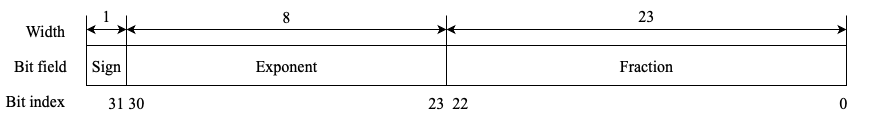
\includegraphics[width=.75\textwidth]{figure1.png}
    \caption{
        Bit-level representation of an IEEE 754 single-precision floating-point 
        number.
    }
\end{figure}

\newpage

The numerical value of this representation is given by the formula:

$$(-1)^s \times M \times 2^{e - \textrm{bias} - p}$$

where $s$ is the sign bit, $M$ is the integral significand (mantissa), $e$ is 
the exponent, and $p$ is the precision of the integral significand. For 
normalized values, the significand $M$ includes an implicit leading 1.

Special cases are determined by the exponent field. If the exponent is all ones, 
the value is either Not a Number (NaN) or infinity. If the exponent is all ones 
and the fraction is zero, the value represents infinity; otherwise, it is NaN. 
If the exponent field is all zeros, the value is denormalized and does not have 
an implicit leading 1.

This report will discuss the implementation details and the underlying
principles of two's complement and floating-point arithmetic as they apply to
modern computer systems.

\section{Implementation}

\subsection{Function \texttt{negate}}

This task requires the implementation of the two's complement unary negation
operator. This is achieved by utilizing the principle of negation in a two's
complement system, which states that the negation of an integer can be
obtained by inverting all of its bits and adding one.

\begin{verbatim}
int negate(int x) { return ~x + 1; }
\end{verbatim}

\subsection{Function \texttt{isLess}}

This function determines if the first argument is less than the second,
returning \verb|1| if true and \verb|0| otherwise. A naive approach using the 
identity $x < y \iff x - y < 0$ is insufficient, as the subtraction may overflow 
in the two's complement system.

Therefore, this implementation first checks if the signs of the arguments
differ. If they do, a negative number is always less than a positive one. If the
signs are the same, the subtraction-based identity is safe to use, as overflow
will not occur.

\begin{verbatim}
int isLess(int x, int y) {
    int sign_diff = ((x ^ y) >> 31) & 1;
    return (sign_diff & !(y >> 31)) |
           ((!sign_diff) & ((x + (~y + 1)) >> 31 & 1));
}
\end{verbatim}

\subsection{Function \texttt{float\_abs}}

The goal of this task is to compute the absolute value of a floating-point 
number by manipulating its bit-level representation. Since the most significant 
bit of a float represents its sign, this can be accomplished by clearing the 
sign bit.

A required edge case is that if the argument is NaN, the function must return 
the argument unmodified. Consequently, the implementation first checks for the 
NaN condition (exponent field is all ones and the fraction is non-zero) before 
proceeding.

\begin{verbatim}
unsigned float_abs(unsigned uf) {
    unsigned mask_exp = 0xFF << 23;

    /* Check if `uf` is NaN. */
    if ((uf & mask_exp) == mask_exp && (uf & 0x007FFFFF) != 0)
        return uf;

    return 0x7FFFFFFF & uf;
}
\end{verbatim}

\subsection{Function \texttt{float\_twice}}

This task requires doubling a floating-point number. The primary strategy is to 
add one to the exponent field. However, several special cases require careful 
consideration.

First, if the input is NaN or infinity, it should be returned unchanged. Second, 
if the input is a denormalized number (including zero), adding one to the 
exponent is incorrect. Instead, the entire number (excluding the sign bit) is 
shifted left by one. Third, if incrementing the exponent of a normalized number 
results in an exponent of all ones, the number has overflowed to infinity, and 
its fraction must be cleared to prevent it from being misinterpreted as a NaN.

\begin{verbatim}
unsigned float_twice(unsigned uf) {
    unsigned mask_exp = 0xFF << 23;
    unsigned exp = uf & mask_exp;

    /* If `exp` is all ones or `uf` is zero, then return `uf` as is since
       multiplying 2 to infinities or NaN would have no effect. */
    if (exp == mask_exp)
        return uf;

    /* If `exp` is zero, then the multiplication by two can be achieved only by
       shifting the number, except the sign bit, to left by one. */
    if (exp == 0)
        return (uf & 0x80000000) | (uf << 1);

    /* If the input is a normal value, multiplication by two is equivalent with
       adding one to the exponent. */
    exp += 1 << 23;

    /* If the incremented result is all ones, the result is overflowed to
       infinity. Zero out the fractional bits to prevent it from being confused
       with NaN. */
    if (exp == mask_exp)
        return (uf & (1 << 31)) | mask_exp;
    else
        return (uf & ~mask_exp) | exp;
}
\end{verbatim}

\subsection{Function \texttt{float\_i2f}}

Converting an integer to a floating-point number is a multi-step process that 
involves determining the final sign, exponent, and fraction, as well as 
performing rounding for values that cannot be represented precisely.

This implementation correctly determines the components and then performs 
rounding according to the **round-to-nearest, ties-to-even** principle. It 
examines the round bit (the first bit shifted out) and the sticky bit 
(the logical OR of all subsequent shifted-out bits) to decide if the fraction 
needs to be incremented. In a tie situation, the final bit of the fraction 
(the guard bit) is checked to ensure the result is even.

\begin{verbatim}
unsigned float_i2f(int x) {
    unsigned frac, exp, round, sticky, increment = 0;

    if (x == 0)
        return 0;

    if (x < 0)
        frac = -x;
    else
        frac = x;

    /* Sum of bias for single-precision floats (127) and 32. */
    exp = 159;

    /* Make sure that MSB of `frac` is 1. */
    while ((frac & 0x80000000) == 0) {
        frac <<= 1;
        exp--;
    }

    /* Shift left once again since floats assume leading zero in its fractional
       bits. Note that we don't have to consider subnormals here since the
       absolute values of all integers, except for zero, is greater than 1
       anyway.*/
    frac <<= 1;
    exp--;

    /* Perform rounding for those numbers that are not exactly representable
       with only 24 bits. */
    round = frac & 0x100;
    sticky = frac & 0xFF;

    if (round && !sticky)
        increment = (frac & 0x200) != 0;
    else if (round && sticky)
        increment = 1;

    frac >>= 9;
    return ((x & 0x80000000) | (exp << 23) | frac) + increment;
}
\end{verbatim}

\subsection{Function \texttt{float\_f2i}}

The conversion from a floating-point number to an integer involves 
reconstructing the integer value from the float's sign, exponent, and fraction. 
The value can be reconstructed by shifting the implicit `1` and the fractional 
bits left by a number of positions dictated by the exponent.

A key aspect of this conversion in C is that it performs **truncation** 
(rounding toward zero). Therefore, no rounding logic is required. After the 
integer part is reconstructed, the final result is obtained by negating it if 
the original float was negative. The implementation also correctly handles 
overflow by returning `0x80000000` for values outside the representable range of 
a 32-bit signed integer.

\begin{verbatim}
int float_f2i(unsigned uf) {
    int exp;
    unsigned integral;

    if ((uf & 0x7FFFFFFF) == 0)
        return 0;

    exp = ((uf & 0x7F800000) >> 23) - 127;

    /* If the exponent is less than zero, than it would be rounded to zero
       anyway. This handles the subnormal case too. */
    if (exp < 0)
        return 0;

    /* Check if the shift by exponent incurs overflow. */
    if (exp >= 31)
        return 0x80000000;

    integral = 1 << exp;
    integral |= (uf & 0x007FFFFF) >> (23 - exp);

    if (uf & 0x80000000)
        return -integral;
    else
        return integral;
}
\end{verbatim}

\section{Result and Discussion}

The execution of the \verb|driver.pl| script confirms that all implemented
functions pass the required correctness and performance tests, achieving a
perfect score.

\begin{verbatim}
[d0319@programming2 datalab2]$ ./driver.pl
...
Score = 31/31 [19/19 Corr + 12/12 Perf] (80 total operators)
\end{verbatim}

The results validate the correctness of the bit-level manipulation strategies 
employed for both two's complement integers and IEEE 754 floating-point numbers. 
The most complex functions, \texttt{float\_i2f} and \texttt{float\_f2i}, 
successfully implemented intricate behaviors like round-to-nearest-even and 
truncation, respectively, demonstrating a comprehensive understanding of data 
representation.

\section{Conclusion}

This assignment was successfully completed, with all functions for manipulating 
integer and floating-point representations meeting the specified correctness and 
performance criteria. The lab provided significant practical insight into the 
low-level mechanics of computer arithmetic.

The primary takeaway from this exercise is the critical role of bit-level 
representation in defining the behavior of numerical operations. Successfully 
implementing functions like \texttt{float\_twice} and \texttt{float\_i2f} 
required moving beyond abstract numerical values to directly manipulating their 
underlying sign, exponent, and fraction fields. This process reinforces the idea 
that for a computer, numbers are not just mathematical concepts but structured 
patterns of bits governed by precise rules.

Furthermore, the assignment highlighted the nuances and edge cases inherent in 
computer arithmetic, such as handling NaNs, infinities, denormalized numbers, 
and overflow conditions. Mastering these details is fundamental to writing 
robust, reliable systems-level code. Ultimately, this lab serves as an effective 
bridge between the theoretical principles of data representation and their 
practical application in software.

\end{document}